\documentclass[border=4pt,12pt]{standalone}
% House style for redrawn exam diagrams (diagram-v4: 0.4pt lines, filled -latex arrows, fine dashes; stipple and hatching drawn as real dots/lines (no PDF/SVG patterns, so they render in every browser and at any scale); transparent background). Every figure \input's this.
\usepackage{amsmath,amssymb}
\usepackage{txfonts}
\usepackage{pdfrender,xcolor}
% \halo{text}: label on shading. The shading stops just around each letter's outline (a thin knock-out that follows the
% glyphs, like the papers' typesetting), never a box. Owner: "I don't want a box around the text".
\newcommand{\halo}[1]{\leavevmode\rlap{\pdfrender{TextRenderingMode=2,LineWidth=2.2pt,LineJoinStyle=1,StrokeColor=white,FillColor=white}#1}#1}
\usepackage{tikz,pgfplots}
\pgfplotsset{compat=1.18}
\usetikzlibrary{arrows.meta,calc,angles,quotes,patterns,patterns.meta,intersections,positioning,decorations.markings,shapes.geometric}
% Stipple and hatching are drawn as actual dots / lines clipped to the region (path picture), NOT as pattern fills:
% SVG <pattern> fills vanish or blur when browsers scale the image, so the owner could not see the shading.
% Each dot is a 0.72pt square (keeps SVGs small; reads as a dot at print size). Dots sit on one global staggered grid, so neighbouring regions line up.
\makeatletter
\newdimen\ex@x \newdimen\ex@y \newdimen\ex@xa \newdimen\ex@ya \newdimen\ex@xb \newdimen\ex@yb \newcount\ex@row
\def\exam@stipplecolor{black!75}\def\exam@dotr{0.42pt}\def\exam@dotgap{2.5}
\def\ex@rowdots{\ifdim\ex@x<\ex@xb \pgfpathrectangle{\pgfqpoint{\dimexpr\ex@x-0.36pt\relax}{\dimexpr\ex@y-0.36pt\relax}}{\pgfqpoint{0.72pt}{0.72pt}}\advance\ex@x by \exam@dotgap pt\relax\expandafter\ex@rowdots\fi}
\def\exam@stipple{%
  \pgftransformreset% dots are sized in real points even inside scaled pictures
  \pgfpointanchor{path picture bounding box}{south west}\ex@xa=\pgf@x \ex@ya=\pgf@y
  \pgfpointanchor{path picture bounding box}{north east}\ex@xb=\pgf@x \ex@yb=\pgf@y
  \pgfsetfillcolor{\exam@stipplecolor}\pgfmathsetmacro\ex@h{\exam@dotgap/2}%
  \pgfmathtruncatemacro\ex@r{floor(\ex@ya/\ex@h)-1}\ex@row=\ex@r\relax
  \ex@y=\ex@r\dimexpr\ex@h pt\relax
  \loop\ifdim\ex@y<\ex@yb
    \pgfmathtruncatemacro\ex@c{floor(\ex@xa/\exam@dotgap)-1}\ex@x=\ex@c\dimexpr\exam@dotgap pt\relax
    \ifodd\ex@row \advance\ex@x by \ex@h pt\fi
    \ex@rowdots
    \advance\ex@y by \ex@h pt \advance\ex@row by 1
    \ifnum\numexpr\ex@row-(\ex@row/4)*4\relax=0 \pgfusepath{fill}\fi% flush every 4 rows: bounded TeX memory, few clip copies in the SVG
  \repeat\pgfusepath{fill}}
\newdimen\ex@d
\def\exam@hatch#1{% #1 = 1 for /, -1 for \ ; lines 45 degrees, 3pt apart
  \pgftransformreset
  \pgfpointanchor{path picture bounding box}{south west}\ex@xa=\pgf@x \ex@ya=\pgf@y
  \pgfpointanchor{path picture bounding box}{north east}\ex@xb=\pgf@x \ex@yb=\pgf@y
  \ex@d=\dimexpr\ex@yb-\ex@ya\relax \ex@x=\dimexpr\ex@xa-\ex@d\relax
  \loop\ifdim\ex@x<\ex@xb
    \ifnum#1>0 \pgfpathmoveto{\pgfqpoint{\ex@x}{\ex@ya}}\pgfpathlineto{\pgfqpoint{\dimexpr\ex@x+\ex@d\relax}{\ex@yb}}%
    \else \pgfpathmoveto{\pgfqpoint{\ex@x}{\ex@yb}}\pgfpathlineto{\pgfqpoint{\dimexpr\ex@x+\ex@d\relax}{\ex@ya}}\fi
    \advance\ex@x by 4.24pt
  \repeat
  \pgfsetlinewidth{0.4pt}\pgfsetstrokecolor{black}\pgfusepath{stroke}}
\def\examstipple{\exam@stipple}\def\examhatch{\exam@hatch}\def\examsetstipplecolor#1{\def\exam@stipplecolor{#1}}\def\examsetdotgap#1{\def\exam@dotgap{#1}}
\makeatother
% (legacy pattern kept for old files)
% staggered stipple like the NESA papers' dotted shading
\pgfdeclarepatternformonly{exam stipple}{\pgfpointorigin}{\pgfqpoint{2.2pt}{2.2pt}}{\pgfqpoint{2.2pt}{2.2pt}}{%
  \pgfpathcircle{\pgfqpoint{0.55pt}{0.55pt}}{0.42pt}\pgfpathcircle{\pgfqpoint{1.65pt}{1.65pt}}{0.42pt}\pgfusepath{fill}}
\tikzset{
  every picture/.style={line width=0.6pt, >={Latex[length=2mm,width=1.3mm]}},
  curve/.style={line width=0.6pt},
  open arrow/.style={-{Latex[length=2mm,width=1.3mm]}},  % owner: filled -latex heads everywhere, no open chevrons
  aux/.style={dash pattern=on 2pt off 1.5pt, line width=0.6pt},
  shade/.code={\def\exA{#1}\def\exB{none}\ifx\exA\exB\else\pgfkeysalso{fill=black!18}\fi},
  shade/.default=on,
  shade dots/.style={fill=none, path picture={\examstipple}},
  stipple color/.code={\examsetstipplecolor{#1}},
  stipple gap/.code={\examsetdotgap{#1}},
  shade dense dots/.style={fill=none, stipple gap=1.6, path picture={\examstipple}},
  shade hatch/.style={fill=none, path picture={\examhatch{1}}},
  shade hatch reverse/.style={fill=none, path picture={\examhatch{-1}}},
  shade solid/.style={fill=black},
  pt/.style={circle, fill, inner sep=1.1pt},
  open pt/.style={circle, draw, fill=white, inner sep=1.1pt},
}
\pgfplotsset{
  exam axes/.style={axis lines=middle, axis line style={->}, xlabel={$x$}, ylabel={$y$},
    xlabel style={anchor=west}, ylabel style={anchor=south}, tick label style={font=\small},
    every axis plot/.append style={line width=0.6pt, black}, samples=200, clip=false,
    enlargelimits=false, axis on top},
}

\usetikzlibrary{decorations.pathmorphing}
\begin{document}
% coordinates in crop pixels (200 dpi), y downward
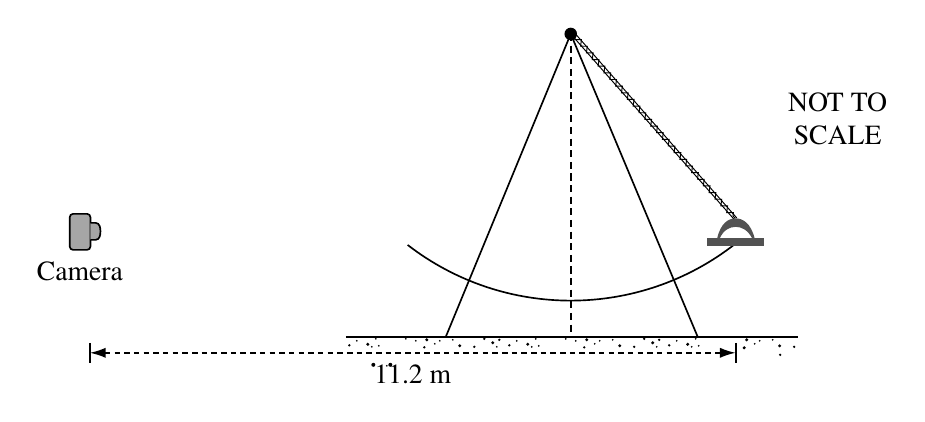
\begin{tikzpicture}[x=0.0127cm, y=-0.0127cm]
  \coordinate (T) at (568,17);
  % ground line and stipple (dot positions taken from the crop)
  \draw (343,320) -- (795,320);
  \foreach \px/\py/\s in {373.0/322.0/1,403.0/322.0/1,424.0/323.0/3,481.5/322.0/2,533.0/322.0/1,563.0/322.0/1,584.0/323.0/3,641.5/322.0/2,693.0/322.0/1,744.0/323.0/3,450.0/323.0/1,496.5/323.0/2,610.0/323.0/1,656.5/323.0/2,770.0/323.0/1,354.0/324.0/1,413.0/324.0/1,437.0/324.0/1,514.0/324.0/1,573.0/324.0/1,597.0/324.0/1,674.0/324.0/1,757.0/324.0/1,490.0/326.0/3,650.0/326.0/3,365.0/327.5/3,432.0/327.0/1,525.0/327.5/3,592.0/327.0/1,685.0/327.5/3,752.0/327.0/1,346.5/328.5/2,457.0/329.0/3,506.5/328.5/2,617.0/329.0/3,666.5/328.5/2,777.0/329.0/3,376.0/329.0/1,536.0/329.0/1,696.0/329.0/1,369.0/330.0/1,421.5/330.5/2,471.5/330.0/2,494.0/330.0/1,529.0/330.0/1,581.5/330.5/2,631.5/330.0/2,654.0/330.0/1,689.0/330.0/1,741.5/331.0/3,791.5/330.0/2,777.5/338.0/2,370.5/348.0/4,387.5/348.0/4,384.0/349.0/1} \fill ({\px},{\py}) circle[radius={0.6+0.35*\s}];
  % swing path arc (centre at pivot)
  \draw[line width=0.6pt] (T) ++(127.7:266.8) arc[start angle=127.7, end angle=52, radius=266.8];
  % frame
  \draw[line width=0.6pt] (443,320) -- (T) -- (695,320);
  \draw[dash pattern=on 2.6pt off 1.6pt, line width=0.6pt] (T) -- (568,320);
  % rope: twisted cord
  \draw[line width=0.35pt] (T) -- (731,202);
  \draw[line width=0.35pt] (571,15) -- (734,201);
  \draw[line width=0.35pt, decorate, decoration={zigzag, segment length=3.2pt, amplitude=0.9pt}] (569.5,16) -- (732.5,201.5);
  % seat: crescent bracket and plank
  \fill[black!68] (714.5,221.5) .. controls (718,206) and (726,201.5) .. (733,201.5)
     .. controls (740,201.5) and (748,206) .. (752,221.5) -- (749.5,221.5)
     .. controls (745,213) and (739,210) .. (733,210) .. controls (727,210) and (721,213) .. (717,221.5) -- cycle;
  \fill[black!68] (704.7,221.3) rectangle (761.3,228.8);
  \node[pt, inner sep=1.6pt] at (T) {};
  % camera
  \draw[fill=black!35, line width=0.6pt, rounded corners=1.2pt] (66.8,197) rectangle (87.5,233);
  \draw[fill=black!35, line width=0.6pt, rounded corners=1.2pt] (87.5,206) -- (96,206) -- (98,214.5) -- (96,223) -- (87.5,223);
  \node at (77,255) {Camera};
  % dimension
  \draw[dash pattern=on 2pt off 1.5pt, line width=0.6pt, {Latex[length=2mm,width=1.3mm]}-{Latex[length=2mm,width=1.3mm]}] (87,336) -- (733,336);
  \draw[line width=0.6pt] (87,326) -- (87,346);
  \draw[line width=0.6pt] (733,326) -- (733,346);
  \node at (410,358) {$11.2$ m};
  \node[align=center] at (835,102) {NOT TO\\SCALE};
\end{tikzpicture}
\end{document}
